\documentclass{beamer}
%PARA VISUALIZAR PRESENTACIONN CON NOTAS USAR VISUALIZADOR "pdfpc":
%Para ver las notas, el cronometro y siguente diapo:
% pdfpc --notes=right slides.pdf
% "tecla p": para pausar el cronometro
\mode<presentation> {
  \usetheme{CambridgeUS}
  \usecolortheme{crane} % color naranja
}
\setbeamercolor{titlelike}{parent=structure,bg=yellow!85!orange} % Cambia el color de la caja del título de la página inicial

\setbeamertemplate{navigation symbols}{} % ocultar iconos de navegación
\setbeamerfont{subsection in toc}{size=\small} % reducir tamaño en TOC
\setbeamerfont{date}{size=\tiny}
\usepackage[spanish]{babel}
\usepackage[utf8]{inputenc}
\usepackage{graphicx}
\usepackage{booktabs}
\usepackage{hyperref}
\usepackage{multicol}
\usepackage{pgfpages}
\usepackage{listings}
\usepackage{multimedia}
\usepackage[export]{adjustbox}
\usepackage{outlines} % Para poner bullets tabulados (\1 \2 \3 ...) y no items

\usepackage{array,tabularx} % para tabular leyenda de ecuaciones
\newenvironment{conditions*} % entorno de "leyenda de ecuación"
  {\par\vspace{\abovedisplayskip}\noindent
   \tabularx{\columnwidth}{>{$}l<{$} @{\ : } >{\raggedright\arraybackslash}X}}
  {\endtabularx\par\vspace{\belowdisplayskip}}
  
% USO DE NOTAS
\setbeameroption{show notes} % Para mostrar u ocultar (hide/show)
%\setbeameroption{show only notes} % Mostrar solo las notas
\setbeameroption{show notes on second screen=right} % Mostrar notas en otra pantalla
\setbeamertemplate{note page}{ % asi solo muestro el texto de las notas
  \insertnote%
}

%========= [TODO]: datos internos del documento
\hypersetup{
	pdftitle={Defensa de trabajo de fin de grado de Unai Sanz Conejo},
	pdfauthor={Unai Sanz Conejo},
	pdfsubject={Flujo de datos en multirobótica},
	pdfkeywords={Programación de flujos de datos, flujos de datos, Zenoh, DDS, ROS2, Zenoh-Flow, Multirobótica, Robótica colaborativa, Robótica móvil, Robótica educativa, Robótica de bajo coste},
	pdfproducer={pdfLaTeX},
  colorlinks=true,
  linkcolor=blue
}
%=========

%========= [TODO]: diapositiva de portada
\title[Flujo de datos en multirobótica]{Flujo de datos en multirobótica} % El título reducido aparece en la parte inferior de todas las diapositivas
%\title[Título reducido]{Título completo}                                % El título completo aparece solo en la diapositiva de portada
\author[Unai Sanz Conejo]{Unai Sanz Conejo}
\institute[URJC]
{
\textit{\href{mailto:u.sanz.2019@alumnos.urjc.es}{\color{blue}{\underline{u.sanz.2019@alumnos.urjc.es}}}}\\
\vspace{0.5cm}

\includegraphics[width=3cm]{figs/logo-urjc}\\
\vspace{1cm}
Trabajo fin de grado
}
\date{4 de Junio de 2024} %[TODO]
%=========

%========= COMIENZO DEL DOCUMENTO
\begin{document}

%========= Portada inicial con notas
\begin{frame}[plain] % plain: quita header y footer
\large{\titlepage}
\note[item]{Muchas gracias, a continuación presentaré mi trabajo de fin de
grado, que como se ha explicado trata sobre la programaciómn de flujos de datos,
sobretodo orientada a entornos educativos, y como se pueden utilizar en conjunto
con ROS2, que, por si no lo conoceis es el middleware de programación en
robótica por excelencia.}
\end{frame}

%========= Licencia
\begin{frame}
% Este diseño se corresponde con la licencia CC-BY-NC-SA.
% Por supuesto, puedes poner la licencia que mejor se adapte al propósito de tu trabajo.
% Recuerda que, si no se especifica ninguna licencia, esta -como cualquier creación artística- pasaría a estar licenciada con todos los derechos reservados (copyright).

\cleardoublepage

\begin{figure}
 \ \ \ \ 
\includegraphics[width=0.25\linewidth]{figs/by-nc-sa.png}
 \label{fig:cc} 
 \end{figure}

\

\

\

\noindent
Este trabajo se distribuye bajo los términos de la licencia internacional \href{http://creativecommons.org/licenses/by-nc-sa/4.0/}{CC BY-NC-SA International License} (Creative Commons AttributionNonCommercial-ShareAlike 4.0). Usted es libre de \textit{(a) compartir}: copiar y redistribuir el material en cualquier medio o formato; y \textit{(b) adaptar}: remezclar, transformar y crear a partir del material. El licenciador no puede revocar estas libertades mientras cumpla con los términos de la licencia:

\begin{itemize}
\item \textit{Atribución}. Usted debe dar crédito de manera adecuada, brindar un enlace a la licencia, e indicar si se han realizado cambios. Puede hacerlo en cualquier forma razonable, pero no de forma tal que sugiera que usted o su uso tienen el apoyo de la licenciante.
\item \textit{No comercial}. Usted no puede hacer uso del material con propósitos comerciales.
\item \textit{Compartir igual}. Si remezcla, transforma o crea a partir del material, debe distribuir su contribución bajo la la misma licencia del original.
\end{itemize}

\begin{flushright}
		\vspace{7.0 cm}
		\emph{Documento de} \textbf{Unai Sanz}. % TODO: pon aquí tu nombre cuando hagas el documento
\end{flushright}


\end{frame}

%========= Índice o tabla de contenidos (TOC)
\begin{frame}
\frametitle{Contenidos}
\begin{multicols}{2} % si tengo muchas secciones, lo parte en dos columnas
  \tableofcontents[hideallsubsections] % no muestra subsecciones
\end{multicols}
\note[item]{La presentación esta dividida en varias partes, en las que
introduciré la robótica dando un contexto general, y explicaré las bases y
aspectos importantes de este proyecto, así como los experimentos y conclusiones
realizadas.}
\end{frame}

% Introducción
% Objetivos
% Plataforma de desarrollo
% Desarrollo Software (Zenoh-Flow + ROS2)
% Pruebas y experimentos
% Conclusiones

%========= Diapositiva "vacía" de comienzo de sección:
\section*{}
\begin{frame}{}
  \centering \Huge
  \emph{Introducción}
\note[item]{Comencemos con la introducción, en la que expondré brevemente el
contexto en la robótica, y sobre todo en los ámbitos más relativos a este
trabajo.}
\end{frame}


\section{Introducción}
\subsection{Contexto general}

%\note[item]{En concreto, la robótica cada vez tiene más importancia en la
%sociedad actual, aplicandose cada vez en más conextos...}

%========= Diapositiva con imágenes:
\begin{frame}
\frametitle{Robótica móvil}
\begin{figure}
\centering
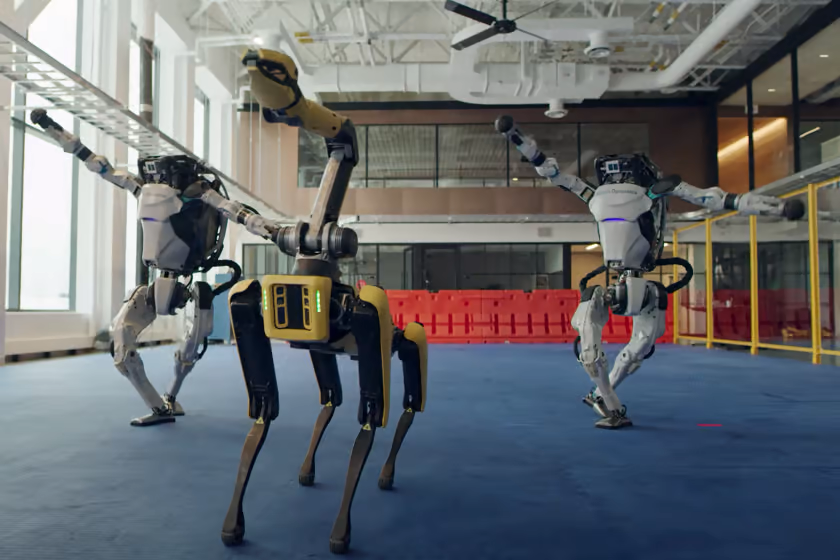
\includegraphics[width=5.0cm]{figs/atlas_spot_robots.png}
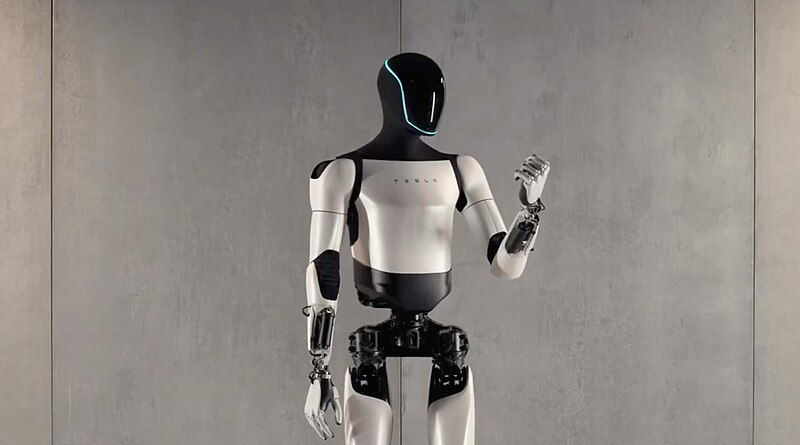
\includegraphics[width=5.0cm]{figs/optimus_tesla.jpg}
\end{figure}
\note[item]{La robótica movil se compone de robots capaces de moverse por el
entorno que les rodea, recopilando información del mismo para tomar sus
decisiones}
\note[item]{Se suelen aplicar en diferentes ámbitos, como en aplicaciones de
búsqueda y rescate, vigilancia, servicios y ocio (robots camareros), industria
militar, etc}
%\begin{figure}
%\centering
%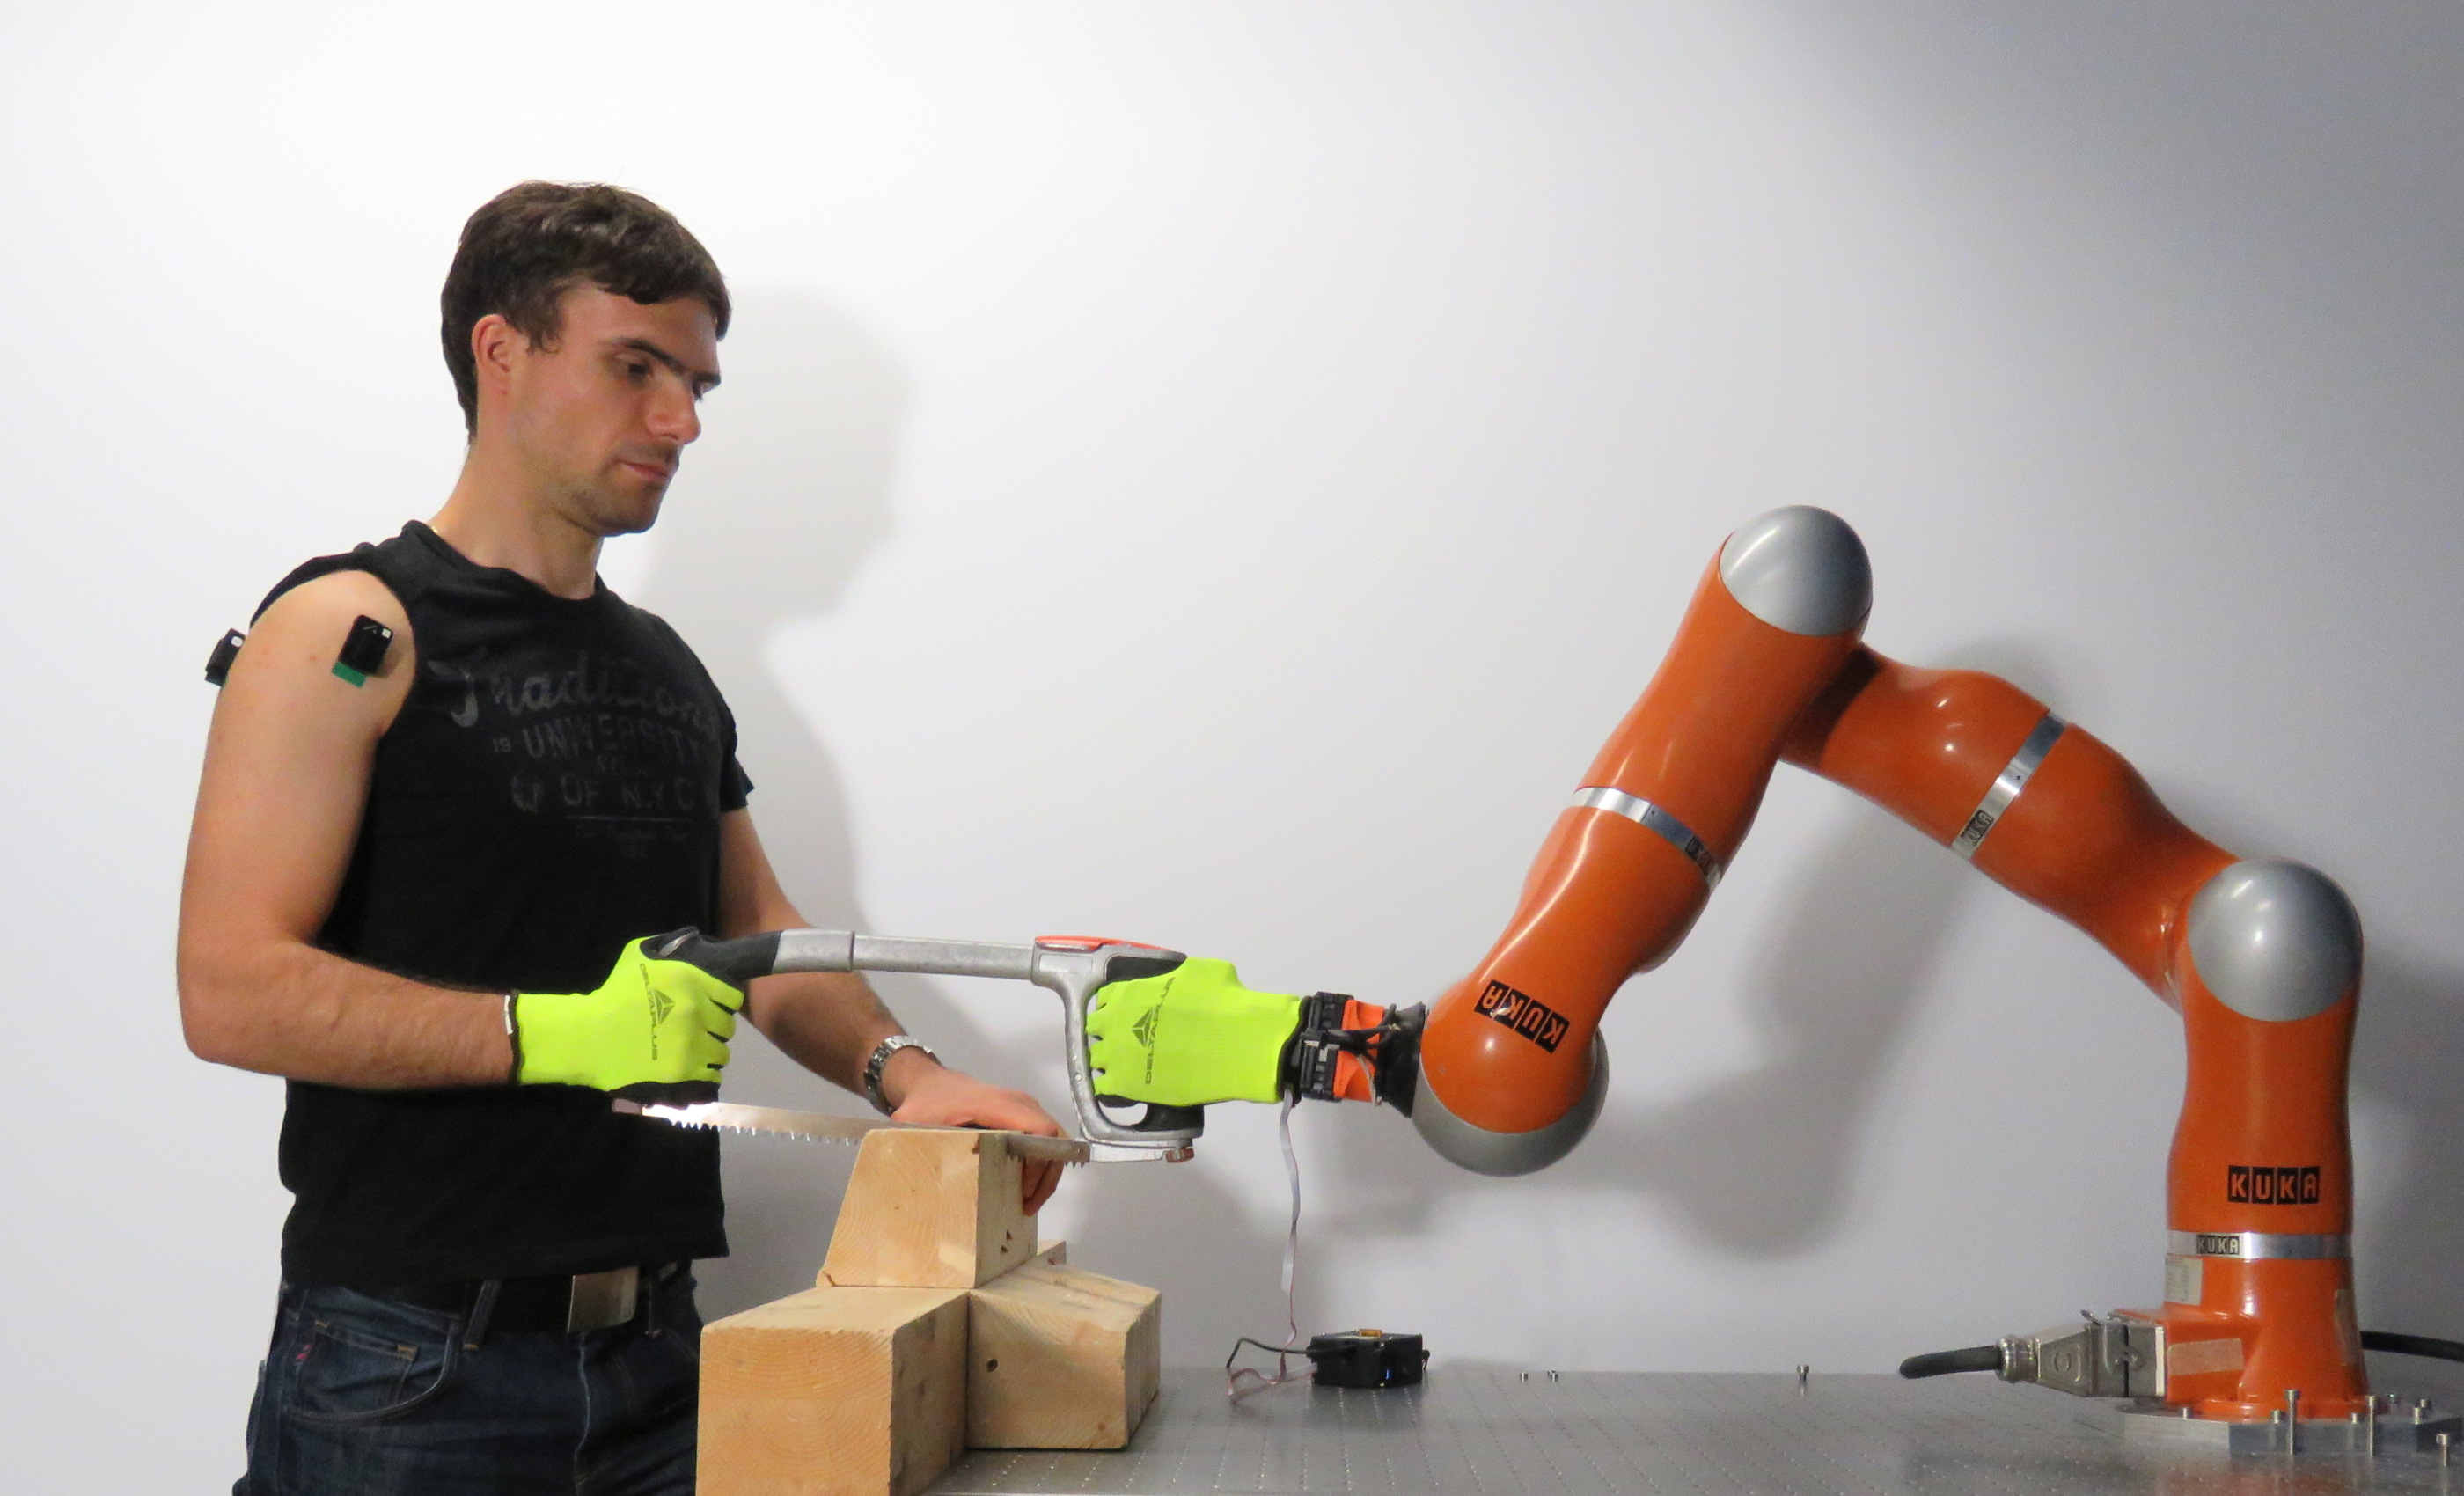
\includegraphics[width=5.0cm]{figs/cobots.jpg}
%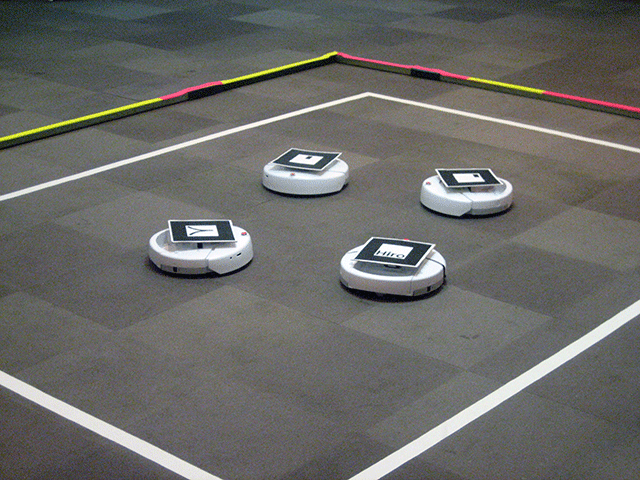
\includegraphics[width=5.0cm]{figs/multirobotics_navigation.png}
%\end{figure}
%\note[item]{Debido en gran medida a este crecimiento de la robótica con ello ha
%surgido la robótica colaborativa y la multrobótica, las cuales me gusta
%diferenciar en cuestión de si ayudan al humano en su tarea o por el contrario la
%realizan de manera autónoma.}
%\note[item]{En este ámbito se encuentra el presente trabajo
%debido a la utilización de múltiples robots para demostrar su desempeño.}
\end{frame}

%========= Diapositiva con imágenes:
\begin{frame}
\frametitle{Robótica educativa y de bajo coste}
\begin{figure}
\centering
a) 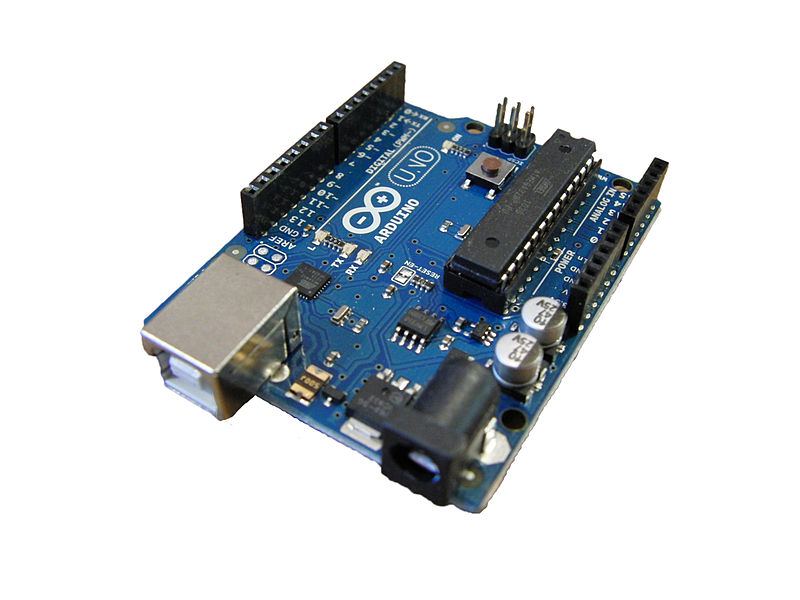
\includegraphics[width=4.0cm]{figs/arduino.jpg}
b) 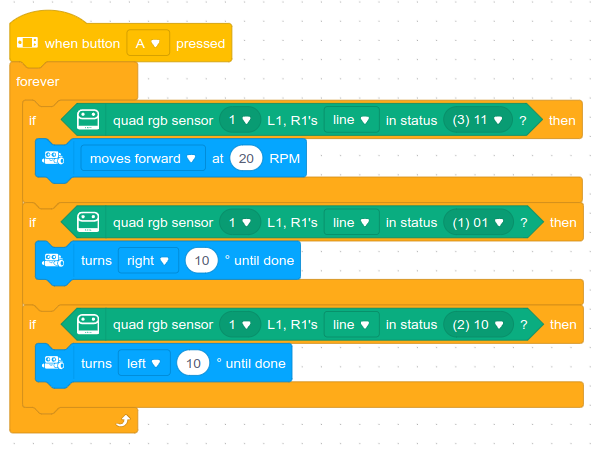
\includegraphics[width=3.5cm]{figs/scratch_arduino_code.png}
c) 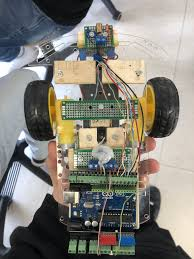
\includegraphics[width=2.5cm]{figs/arduino_bot.jpeg}
\end{figure}
\begin{figure}
\centering
d) 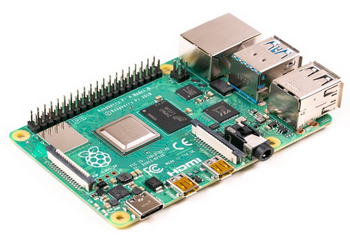
\includegraphics[width=4.0cm]{figs/raspberry_pi_4b.png}
%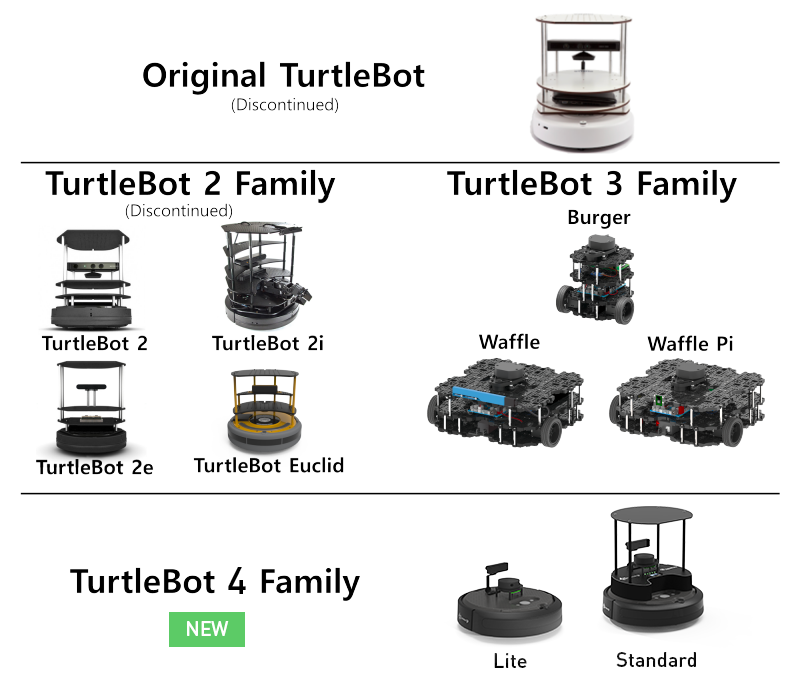
\includegraphics[width=5.0cm]{figs/turtlebot_family.png}
e) \includegraphics[width=4.0cm]{figs/multirobotics_education.jpg}
\end{figure}
\note[item]{En relacion con el anterior campo de la robótica, la educación cobra
un papel importante dado el crecimiento de este ámbito, por lo que cada vez es
más importante su enseñanza}
\note[item]{Para ello la investigación se ha encargado de desarrollar la
robótica de bajo coste, que se nutre de placas más económicas para entidades
como institutos, y que se llevan utilizando en el itinerario formativo en España
desde 2015}
\note[item]{Algunos de estos ejemplos... (imágenes)}
\end{frame}

%========= Diapositiva con imágenes:
\begin{frame}
\frametitle{Robótica colaborativa}
\begin{figure}
\centering
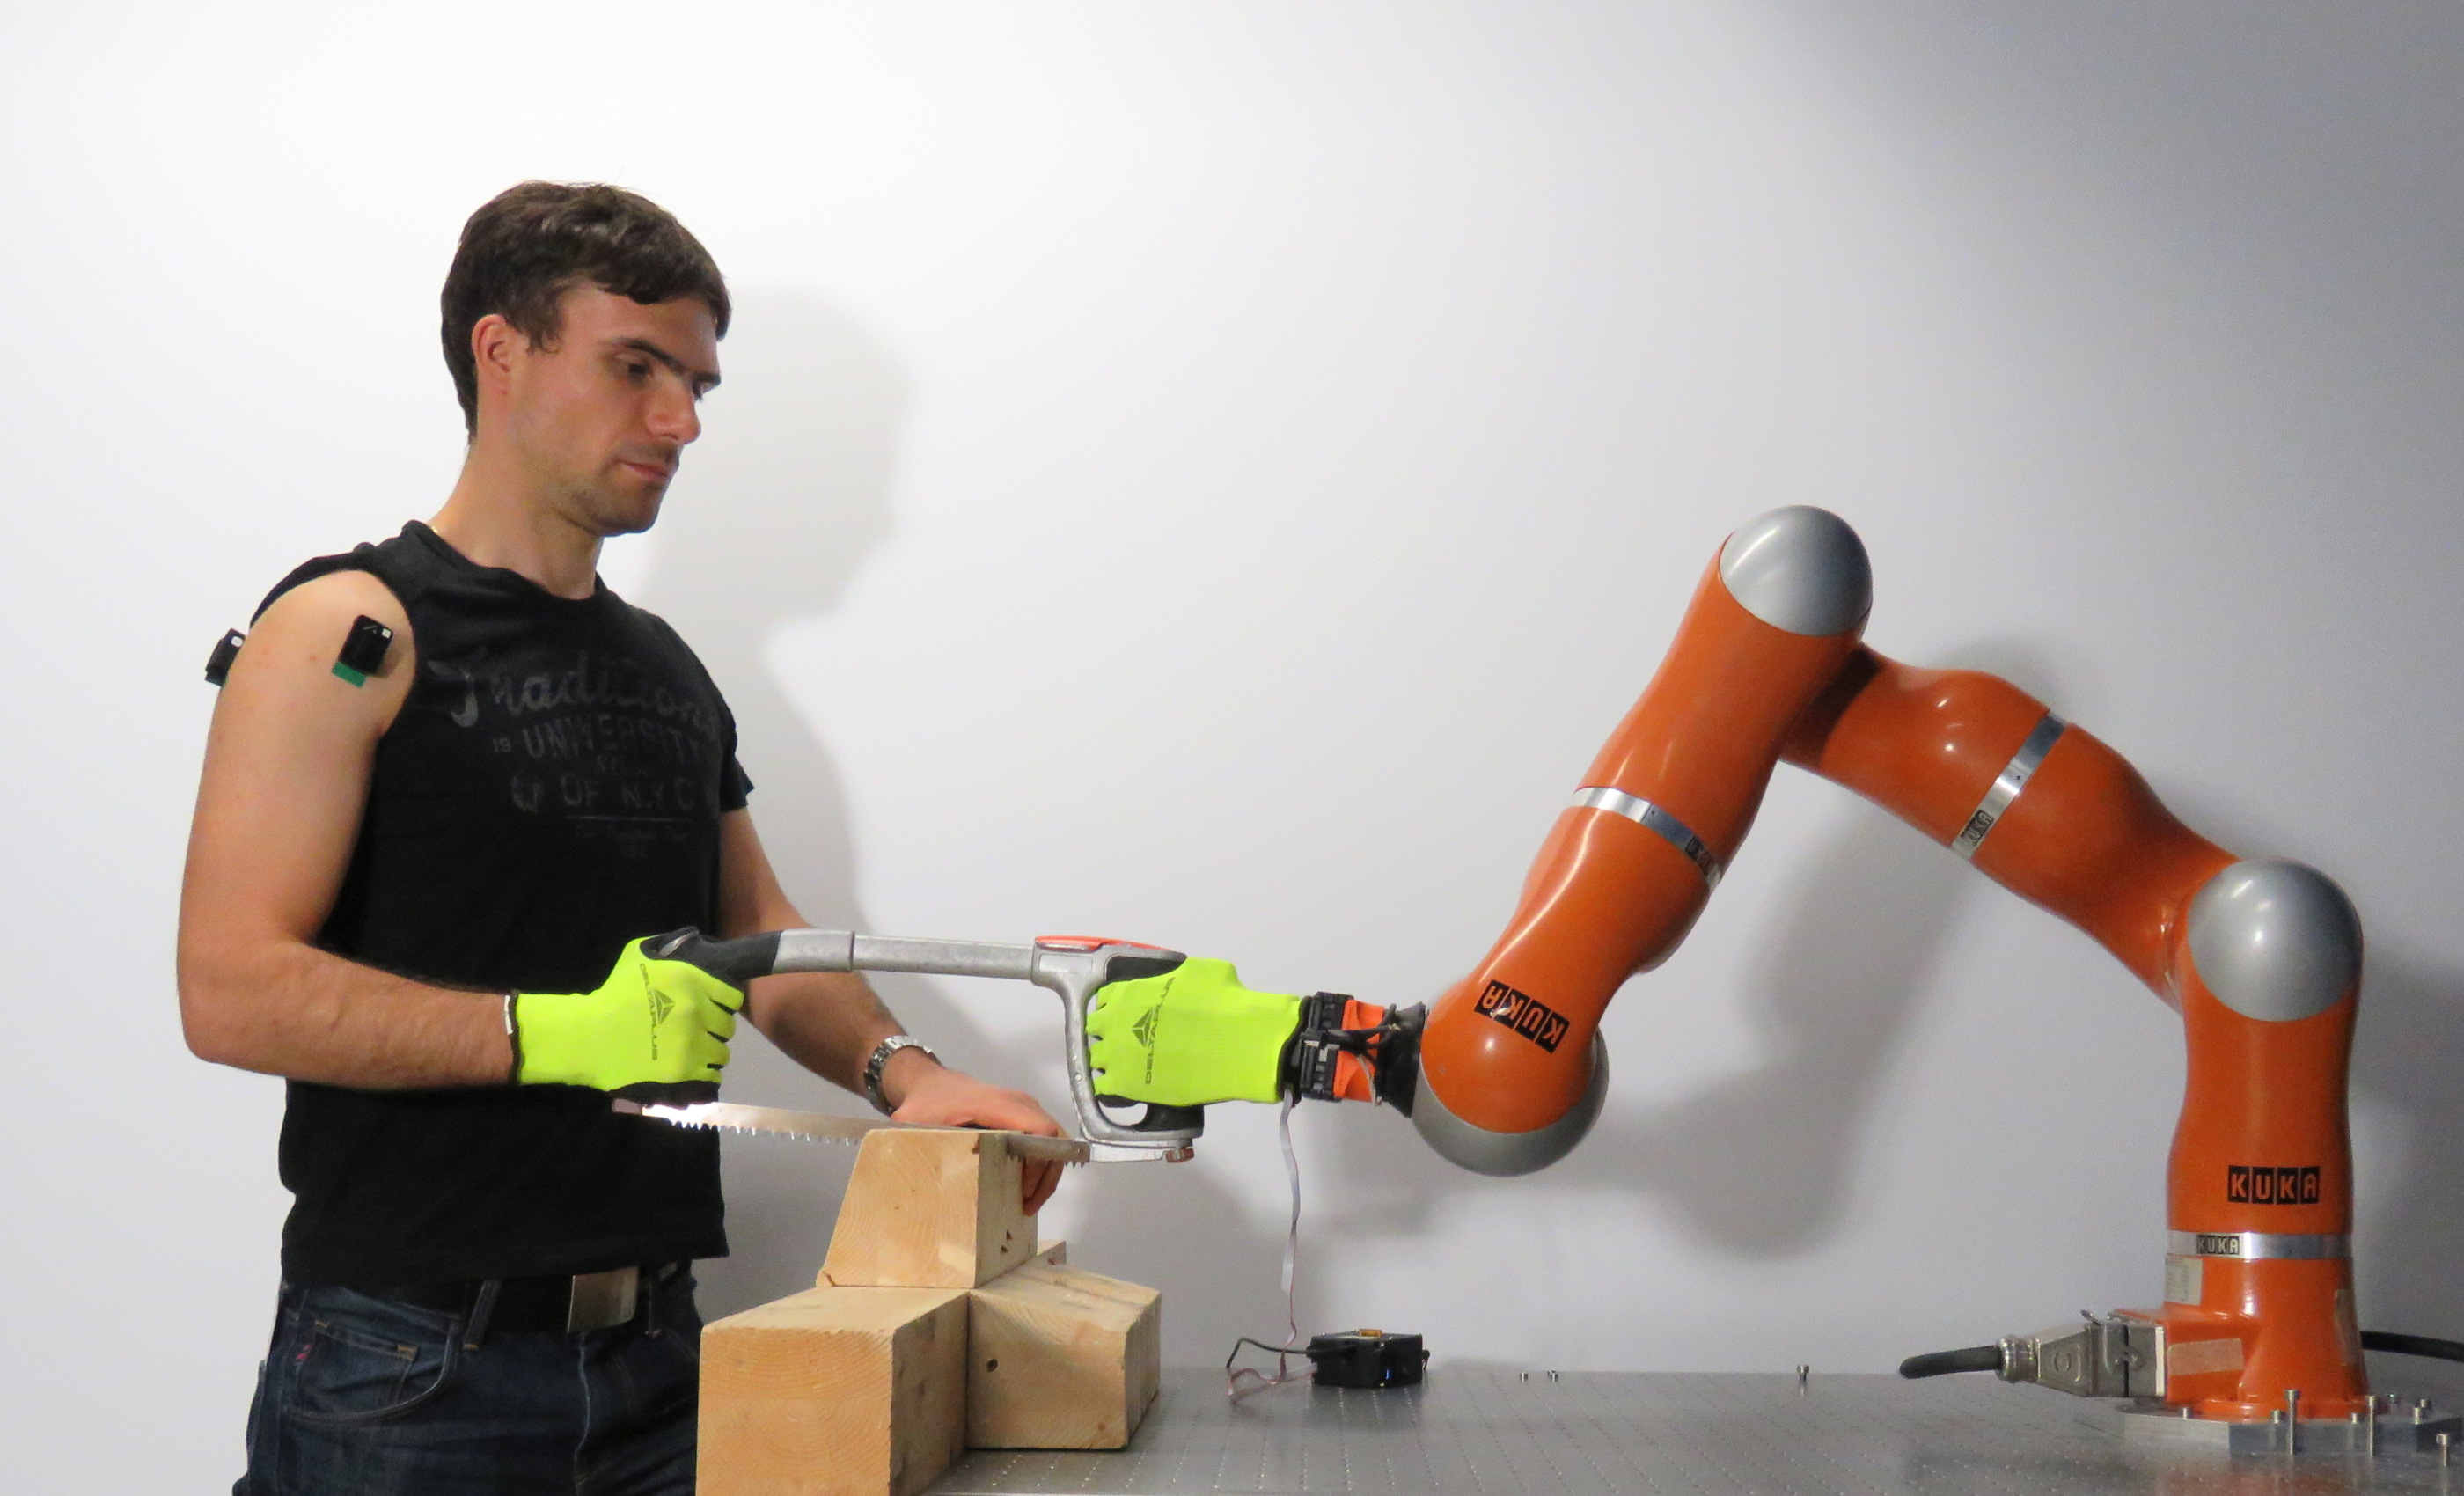
\includegraphics[width=5.0cm]{figs/cobots.jpg}
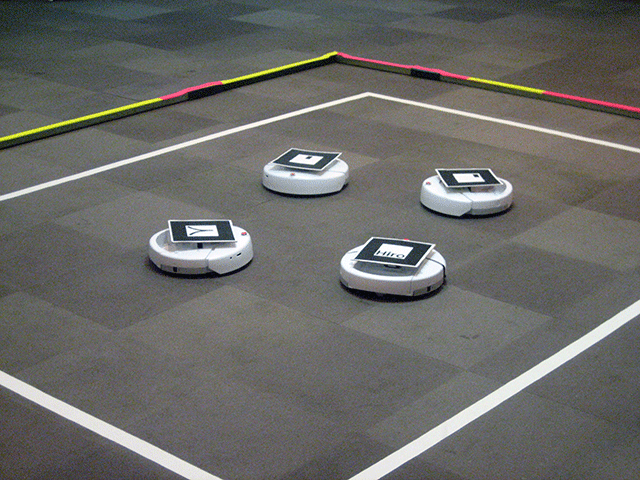
\includegraphics[width=5.0cm]{figs/multirobotics_navigation.png}
\end{figure}
\note[item]{Debido en gran medida a este crecimiento de la robótica con ello ha
surgido la robótica colaborativa y la multrobótica, las cuales me gusta
diferenciar en cuestión de si ayudan al humano en su tarea o por el contrario la
realizan de manera autónoma.}
\note[item]{En este ámbito se encuentra el presente trabajo
debido a la utilización de múltiples robots para demostrar su desempeño.}
\end{frame}

\begin{frame}
\frametitle{Flujos de datos en robótica}
\begin{block}{Comparación \textcolor{red}{Robots} con \textcolor{blue}{Flujos de datos}}
\begin{outline}
\1 \textcolor{red}{Sensores} = nodo \textcolor{blue}{Source}.
\1 \textcolor{red}{Cómputo} = nodo \textcolor{blue}{Operator}.
\1 \textcolor{red}{Actuadores} = nodo \textcolor{blue}{Sink}.
\end{outline}
\end{block}
\begin{figure}
\centering
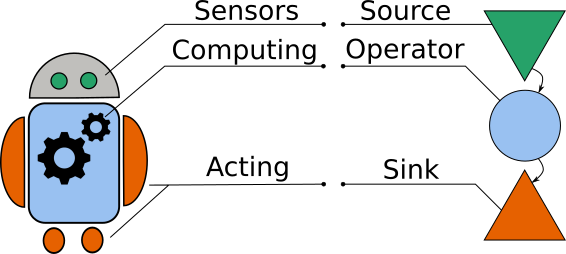
\includegraphics[width=8.0cm]{figs/data-flow_vs_robotics_scheme.png}
\end{figure}
\note[item]{Los flujos de datos suelen componerse de 3 nodos, el primero en el
que se originan los datos, al que llamaremos sink, el segundo donde se computan,
al que llamaremos operator, y el último en el que los datos terminan su paso por
el flujo, y aplicado a la robótica, muchas veces se acaban convirtiendo en
decisiones o acciones tomadas por el robot.}
\note[item]{Como se puede observar en la imagen, la similitud entre los propios
componentes del robot y los de un flujo de datos es amplia, haciendo que su
aplicación sea sencilla en este ámbito, sobretodo asemejando un comportamiento
reactivo del robot, en el que se actúa en función de los datos recibidos, y que
suele ser la forma más básica de programación de los robots durante su
aprendizaje.}
\note[item]{El hecho de aplicar los flujos de datos como forma de programación
lo convierte en un paradigma de programación en sí mismo.}
\end{frame}

%========= Diapositiva con imágenes:
%\begin{frame}
%\frametitle{Ejemplo de flujo de datos}
%\begin{figure}
%\centering
%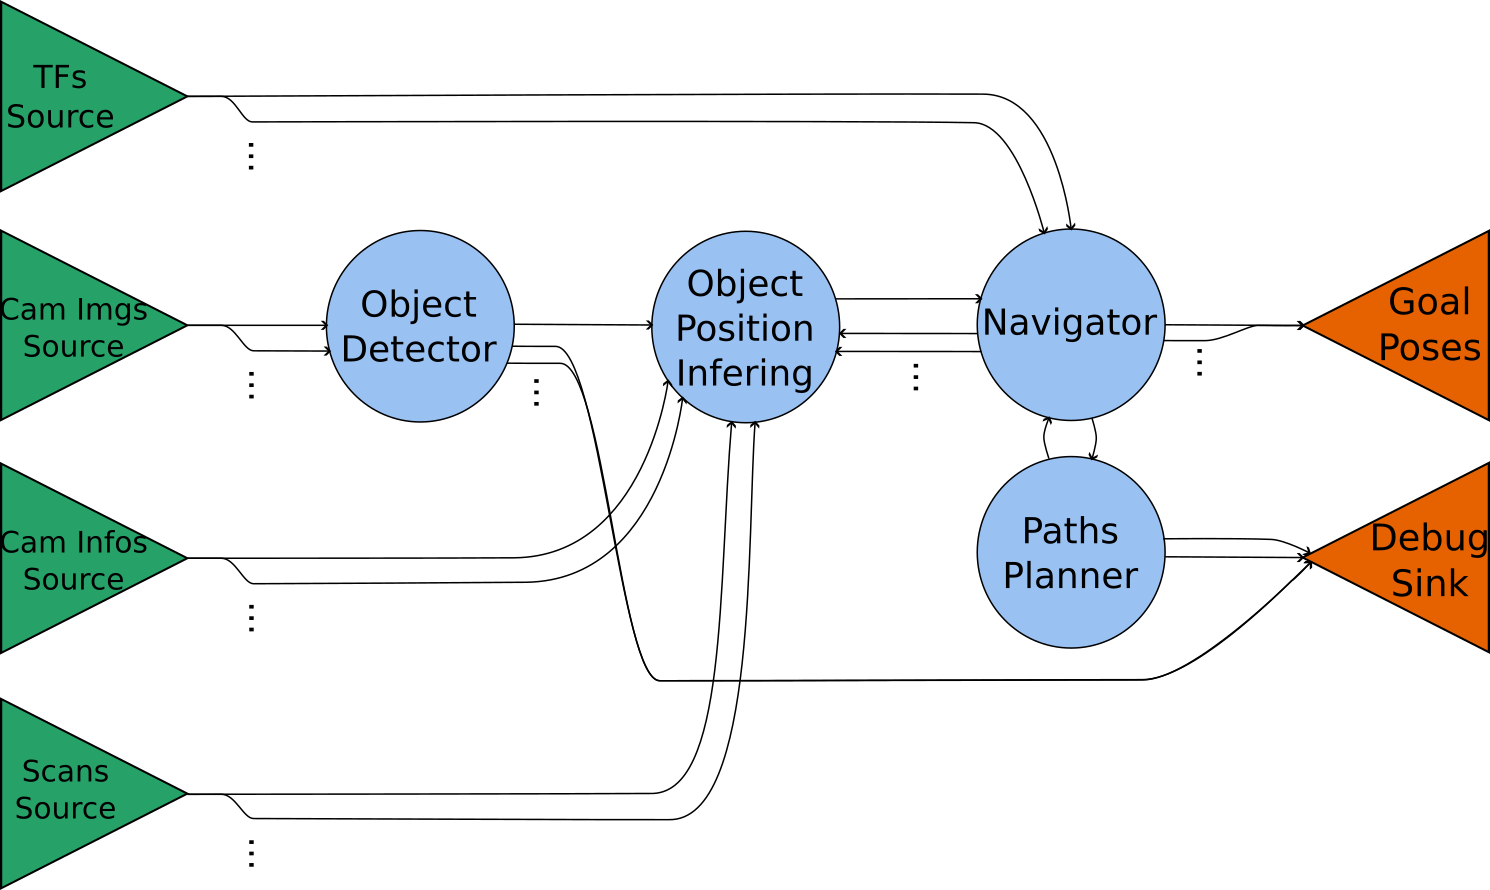
\includegraphics[width=10.0cm]{figs/data_flow_scheme.png}
%\end{figure}
%\note[item]{Con este contexto podemos visualizar un flujo de datos como una red
%de nodos que forman un grafo dirigido, en el que los datos fluyen entre dichos
%nodos.}
%\note[item]{En la imagen podemos ver un ejemplo de uno de ellos, concretamente
%de la aplicacaión desarrollada para este proyecto, basada en la búsqueda de un
%objeto en una sala por múltiples robots.}
%\end{frame}





%========= Diapositiva "vacía" de comienzo de sección:
\section*{}
\begin{frame}{}
  \centering \Huge
  \emph{Objetivos}
\note[item]{Comencemos con los objetivos.}
\end{frame}

\section{Objetivos}
%\subsection{Descripción del problema}
%========= Diapositiva con bullets en diferentes niveles (outline) e imágenes:
\begin{frame}
\frametitle{Descripción del problema}
\begin{block}{Problemas}
\begin{outline}
\1 \textcolor{red}{Congestion} de red
  \2 Generada por \textcolor{blue}{DDS}.
\1 \textcolor{red}{Escalón de aprendizaje} en robótica.
  \2 Dificultad de \textcolor{blue}{ROS}.
\end{outline}
\end{block}
\begin{figure}
\centering
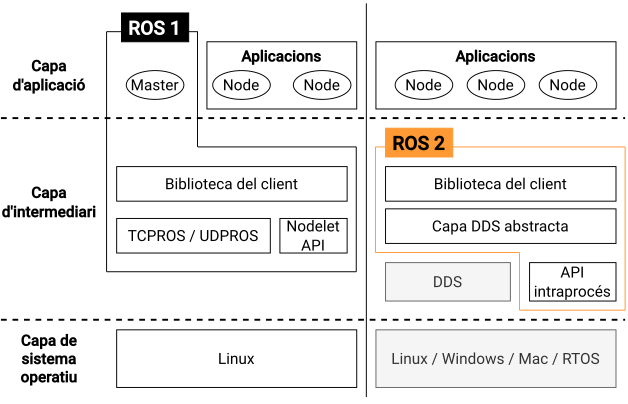
\includegraphics[width=6.0cm]{figs/ROS_and_ROS2.png} %[TODO] ¿Alomejor cambiar por imagen sobre congestion de red?
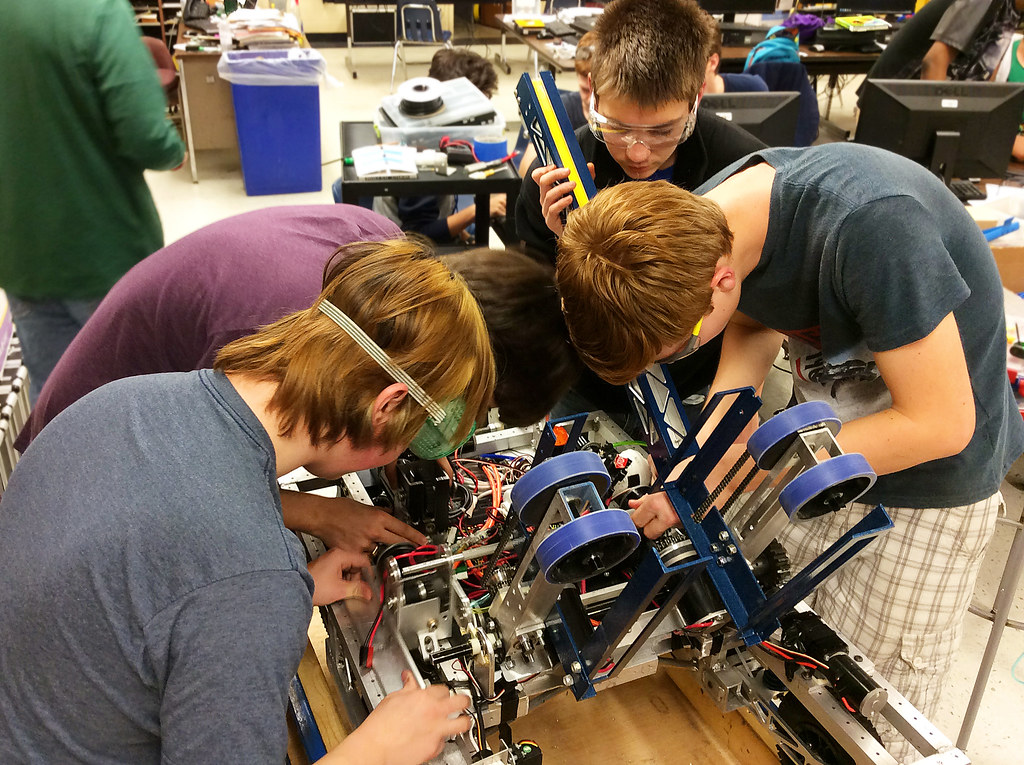
\includegraphics[width=4.5cm]{figs/robotics_students.jpg}
\end{figure}
\note[item]{Un gran problema de la robótica actualmente surge debido al envío de
gran cantidad de mensajes entre los robots, especialmente en multirobótica, que
en muchos casos, se ve incrementado por el envío de mensajes de Discovery con la
utilización de DDS como protocolo de comunicaciones.}
\note[item]{En relación con la educación, los alumnos preuniversitarios, que en
su mayoría provienen de un sistema mucho más básico, de placas sencillas,
entornos de programación visuales y hardware básico, encuentran un escalón de
aprendizaje debido al uso de ROS y su gran dificultad, propiciado por el entorno
que lo rodea, que requiere conceptos e ideas nuevas para su comprensión por
parte del alumnado.}
\note[item]{Es por este motivo que la solución propuesta se basa en la sencillez
de entendimiento y programación del código así como en la reducción de la
congestión de red, lo que además brinda un entorno de programación más simple, a
la vez que compatible con el uso de nodos existentes de ROS, adquiriendo sus
ventajas y paliando sus desventajas.}
\end{frame}


%[TODO] Trasparencia de Plantemiento de solución.


%\subsection{Descripción del problema}
%========= Diapositiva con bullets (outline):
\begin{frame}
\frametitle{Requisitos}
\begin{block}{}
\begin{outline}
\1 \textcolor{red}{Ubuntu 22.04} LTS en todas las máquinas.
\1 \textcolor{red}{Compatibilidad} entre herramientas software.
\1 \textcolor{red}{Facilidad de reproducción y despliegue}.
\1 \textcolor{red}{Sencillez} de las aplicaciones robóticas desarrolladas.
\1 Hardware \textcolor{red}{económico}.
\end{outline}
\end{block}
\note[item]{De esta manera los requisitos propuestos pasan por la facilidad de
reproducción y despliegue en un entorno de laboratorio, la sencillez de
programación, la compatibilidad entre softwares, y un la posibilidad de
aplicación sobre un hardware económico brindado por la escuela o instituto
objetivo.}
\end{frame}

\begin{frame}
\frametitle{Metodología}
\begin{block}{}
\begin{outline}
\1 Ciclo de desarrollo software \textcolor{red}{iterativo}.
  \2 Actualizaciones en \textcolor{blue}{YouTube} y \textcolor{blue}{GitHub} \textcolor{red}{\url{https://github.com/RoboticsURJC/tfg-unai}}.
\1 \textcolor{red}{Reuniones} semanales.
\1 Desarrollo de la \textcolor{red}{memoria}.
\end{outline}
\end{block}
\begin{figure}
\centering
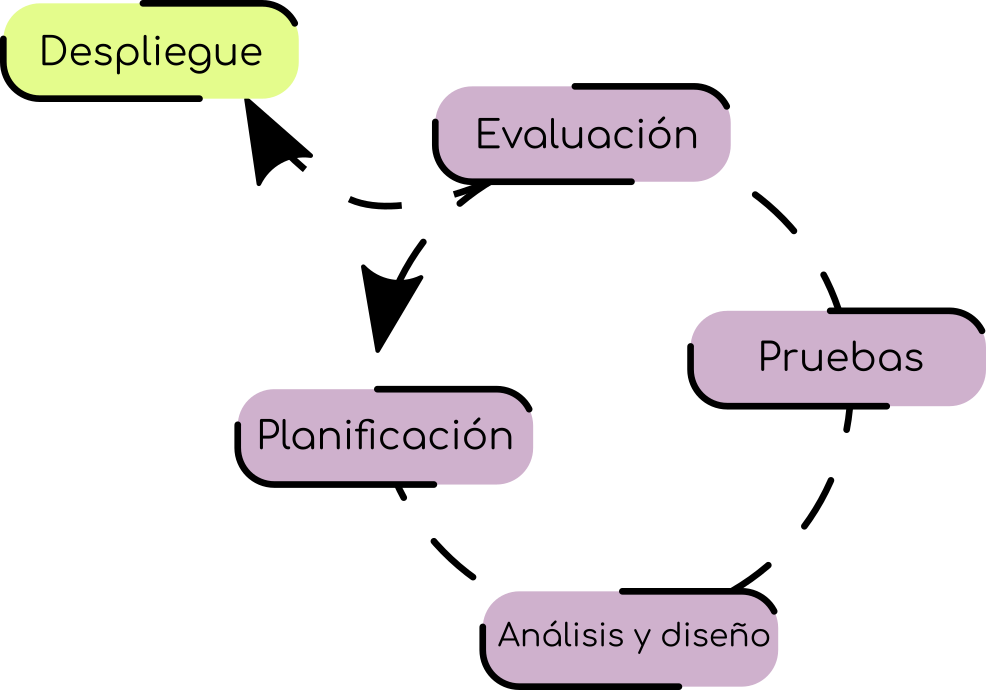
\includegraphics[width=6.0cm]{figs/desarrollo_iterativo.png}
%[TODO] ¿Alomejor añadir imagen sobre congestion de red?
\end{figure}
\note[item]{Para el cumplimiento de estos requisitos así como el desarrollo de
la aplicacaioón demostrativa, se utilizó un método iterativo de desarrollo
software, que pasa por la mejora continua del programa hasta su versión final.}
\note[item]{Asímismo se desarrolló una memoria, y documentación del proyecto
tanto en GitHub como en Youtube, así como se mantuvieron reuniones semanales con
el tutor.}
\end{frame}





%========= Diapositiva "vacía" de comienzo de sección:
\section*{}
\begin{frame}{}
  \centering \Huge
  \emph{Plataforma de desarrollo}
\note[item]{Comencemos con la plataforma de desarrollo.}
\end{frame}

\section{Plataforma de desarrollo}
%\subsection{}

\begin{frame}
\frametitle{Hardware}
\begin{figure}
\centering
\includegraphics[width=3.4cm]{figs/multirobotics_education.jpg}
\end{figure}
\begin{figure}
\centering
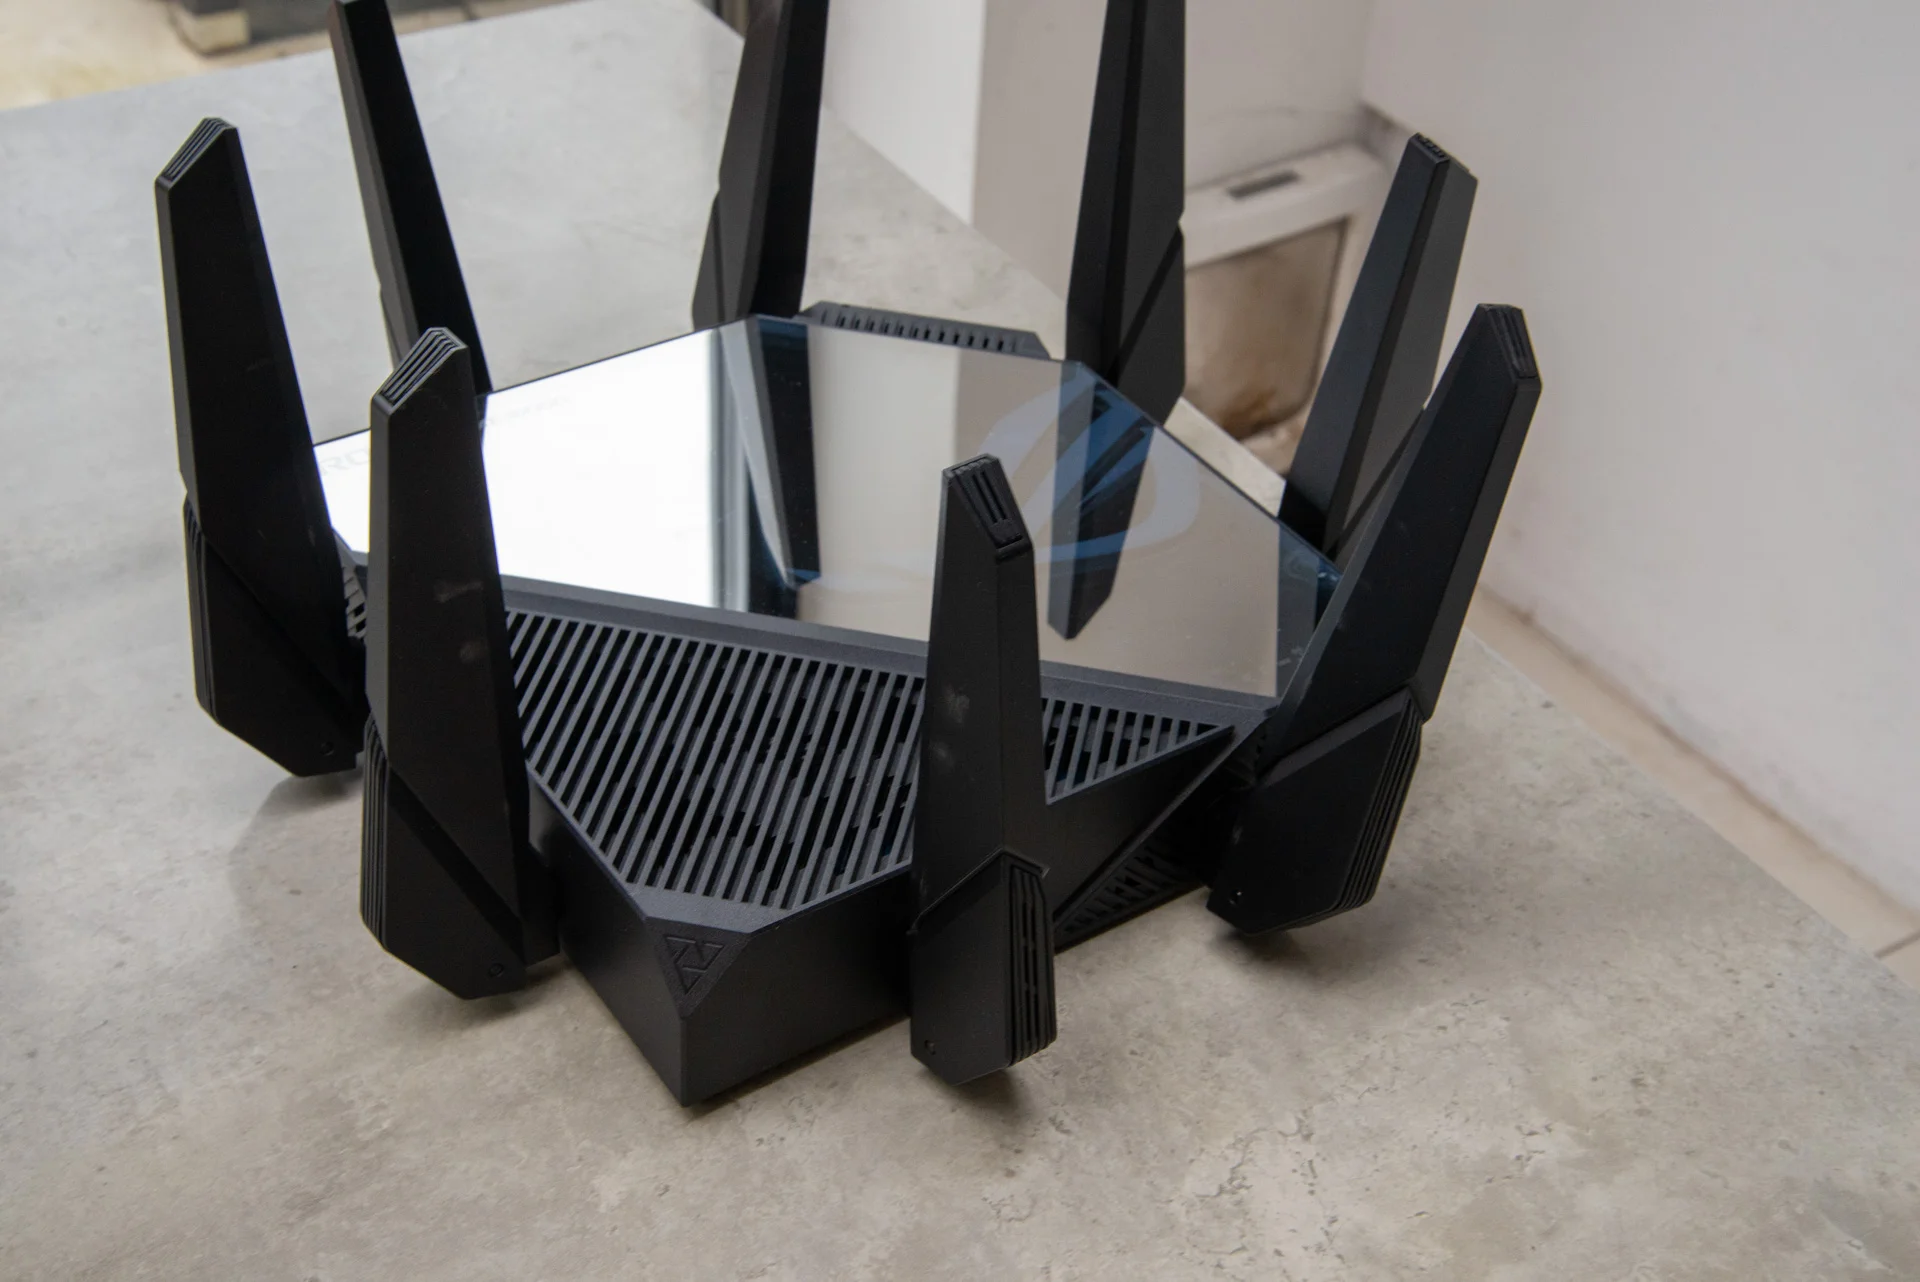
\includegraphics[width=3.4cm]{figs/asus_router.png}
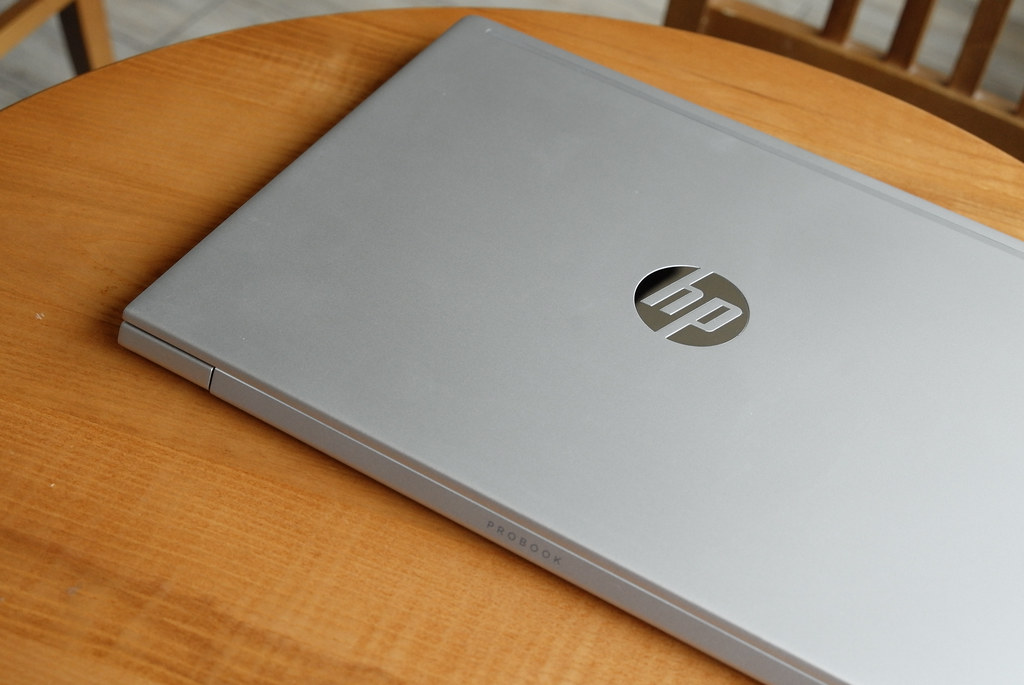
\includegraphics[width=3.4cm]{figs/hp_probook.jpg}
\end{figure}
\note[item]{En cuanto a la plataforma de desarrollo hardware, se utilizaron los
robots del laboratorio de robótica de la URJC (T2 y T4 Lite), así como el
router allí desplegado y un portátil HP con capacidad suficiente (16GB RAM)
para la ejecución de todos los nodos.}
\note[item]{Además dicho portatil compone el ordenador de abordo del robot T2
utilizado, mientras que los T4 utilizan homónimamente una Raspberry Pi 4B.}
\end{frame}

\begin{frame}
\frametitle{Software}
\begin{figure}
\centering
a) 
\includegraphics[width=2.5cm]{figs/ros2_humble_logo.png}
b) 
\includegraphics[width=2.5cm]{figs/zenoh_logo.png}
c) 
\includegraphics[width=2.5cm]{figs/nav2_logo.png}
\end{figure}
\begin{figure}
\centering
d) 
\includegraphics[width=2.5cm]{figs/gazebo_logo.png}
e) 
\includegraphics[width=2.5cm]{figs/python_logo.png}
f) 
\includegraphics[width=2.5cm]{figs/opencv_logo.png}
\end{figure}
\note[item]{En cuanto al software utilizado podemos nombrar ROS2 Humble, el
stack de navegación (Nav2), Zenoh y softwares relativos como Zenoh-Flow,
Zenoh-bridge-DDS, además de OpenCV para la detección, Gazebo para la simulación
y Python como lenguage de pogramación para el desarrollo de la aplicación
demostrativa.}
\end{frame}





%========= Diapositiva "vacía" de comienzo de sección:
\section*{}
\begin{frame}{}
  \centering \Huge
  \emph{Arquitectura Software}
\note[item]{Comencemos con la arquitectura software.}
\end{frame}

\section{Arquitectura Software}
\subsection{Topología}

\begin{frame}
\frametitle{Topología hardware}
\begin{block}{Características}
\begin{outline}
\1 Red \textcolor{red}{sin} necesidad de acceso a \textcolor{red}{Internet}.
\1 Topología \textcolor{red}{centralizada} alrededor del portátil.
  \2 Máquina más potente que correrá todo el software.
\end{outline}
\end{block}
\begin{figure}
\centering
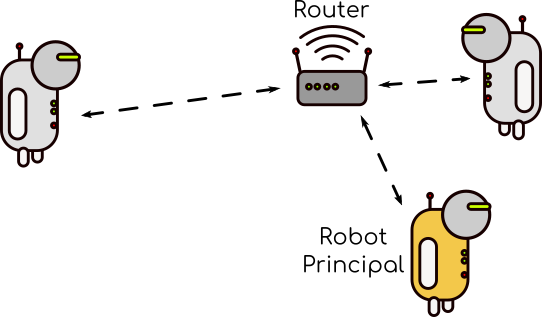
\includegraphics[width=4.0cm]{figs/network_topology.png}
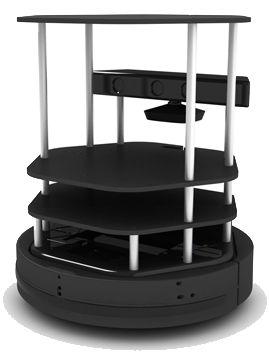
\includegraphics[width=2.5cm]{figs/turtlebot2.png}
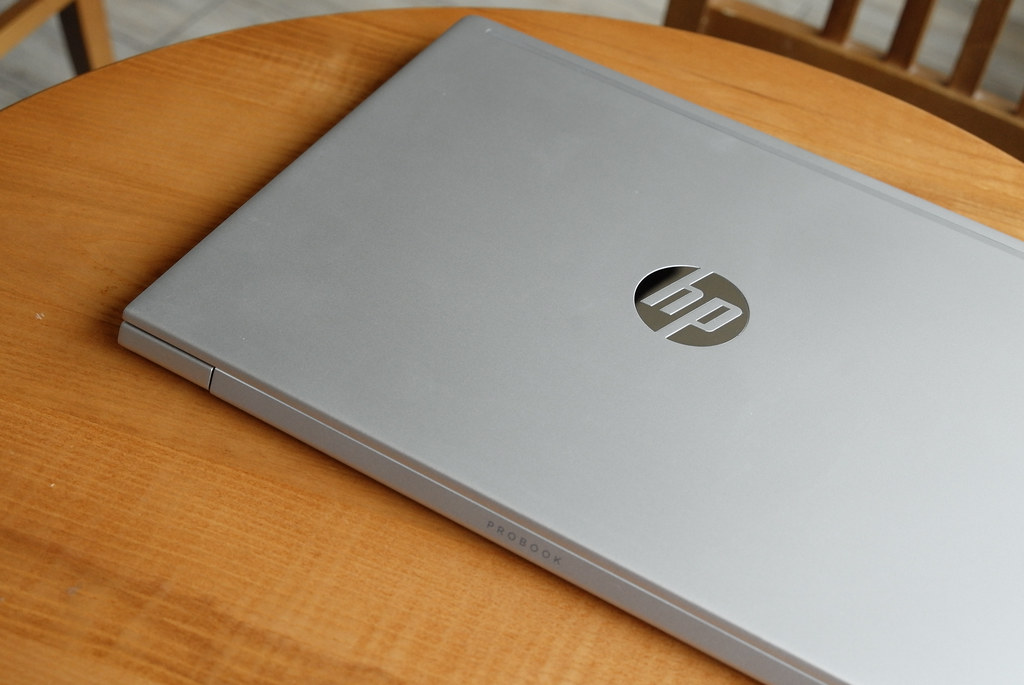
\includegraphics[width=4.0cm]{figs/hp_probook.jpg}
\end{figure}
\note[item]{La distriucicón del harware en la red es equitativo, estando ambos
robots y ordenadores de a bordo en la misma sala, permitiendo su comunicación
mediante el router como intermediario y sin necesidad de acceso a internet.}
\note[item]{Además, como ya hemos explicado previamente, el portátil correrá la
mayoría del software, por lo que topológicamente hablando, es el principal.}
\end{frame}

\begin{frame}
\frametitle{Topología software}
\begin{block}{Características}
\begin{outline}
\1 \textcolor{red}{División} en nodos.
\1 \textcolor{red}{Modularización} del código.
\end{outline}
\end{block}
%\begin{figure}
%\centering
%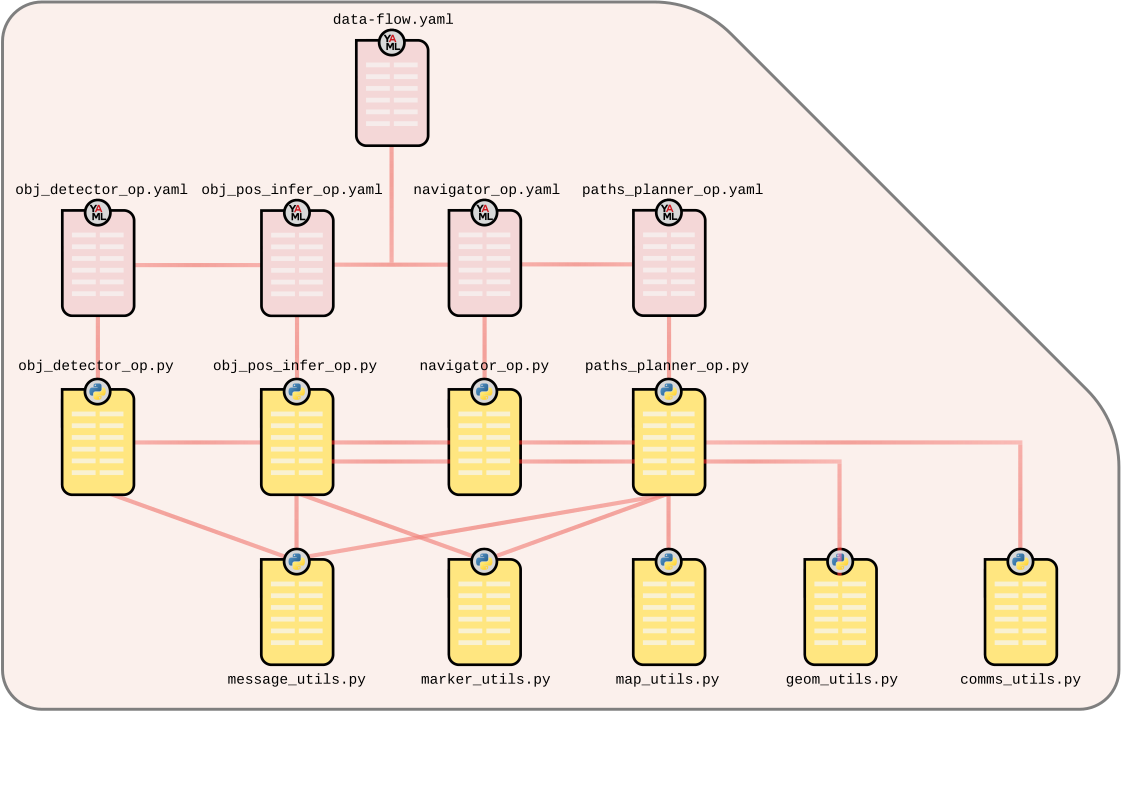
\includegraphics[width=6.0cm]{figs/files_scheme.png}
%\end{figure}
\begin{figure}
\centering
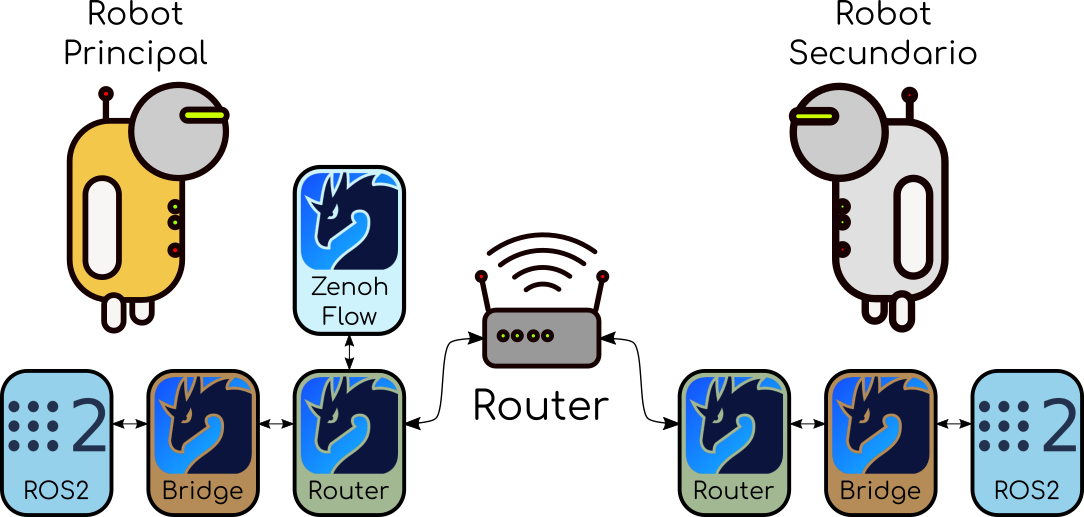
\includegraphics[width=10.0cm]{figs/software_tools_architecture.png}
\end{figure}
%[TODO] Añadir imagen que muestre la topologia software a nivel de que robot
%       corre zenoh y zenoh-bridge-dds, cual zenoh-flow ademas de los anteriores
\note[item]{En cuanto al software,  como se puede observar en la imagen, este
trabajo se compone en su base de nodos de ROS2 (DDS), que se pueden comunicar
con los nodos de Zenoh-Flow (Zenoh) mediante el Zenoh-bridge-DDS, encargado de
traducir los mensajes.}
\note[item]{Asímismo, se necesitan routers de zenoh corriendo en cada máquina
para que estas puedan recibir los mensajes de Zenoh enviados por Zenoh-Flow
desde la máquina principal y traducirlos mediante el uso del bridge a DDS, y
poder así comunicarse con los nodos de ROS2.}

%[TODO] Mover la imagen de los archivos y el siguiente texto a posteriores
%       trasparencias para explicar como funciona un flujo de datos en
%       Zenoh-Flow y su sencillez/complejidad segun la necesidad de la
%       aplicación.
%\note[item]{Como podemos observar en la imagen, la estructura de archivos de la
%aplicación desarrollada puede ser escalada de manera más compleja, aunque lo
%único necesario para poder hacer funcionar un flujo de datos en Zenoh-flow son 2
%archivos, uno de ellos yaml, y el otro deberá contener una clase sencilla de
%Python, por lo que se puede llegar a convertir en todo lo simple o complejo que
%se requiera en cada aplicación, dandoa demás la libertad de eliminar o añadir
%nodos fácilmente.}
\end{frame}





%[TODO] Tal vez los flujos de datos no deberian tener seccion propia? (yo creo que sí)

%========= Diapositiva "vacía" de comienzo de sección:
\section*{}
\begin{frame}{}
  \centering \Huge
  \emph{Desarrollo}
\note[item]{Comencemos con la rogramación de flujos de datos.}
\end{frame}

\section{Programación de flujos de datos con Zenoh-Flow y ROS2}
\subsection{Flujos de datos}



%[TODO] Hablar en las notas sobre cómo se realiza la serialización de los mensajes (/rt/ y serializadores internos de ROS)
\subsection*{}
\begin{frame}
\frametitle{Programación de flujo de datos}
\begin{block}{Componentes software}
\begin{outline}
\1 \textcolor{red}{Zenoh}            (\textcolor{blue}{protocolo} de comunicaciones).
\1 \textcolor{red}{Zenoh-Flow}       (\textcolor{blue}{framework} para programación de flujos de datos).
\1 \textcolor{red}{Zenoh-bridge-DDS} (\textcolor{blue}{traductor} Zenoh-DDS).
\end{outline}
\end{block}
\begin{figure}
\centering
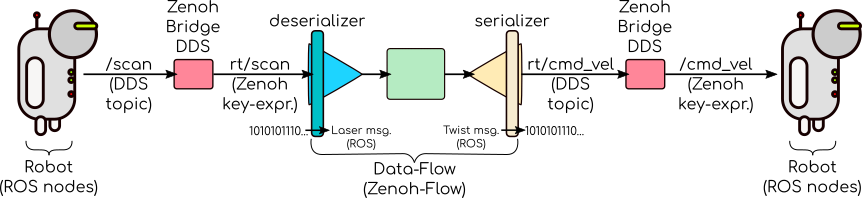
\includegraphics[width=12.0cm]{figs/zenoh_dds_topology.png}
\end{figure}
\note[item]{La siguiente imagen representa la forma de aplicar este paradigma de
programación junto con ROS2, ejecutando el flujo de datos con Zenoh-Flow, y
utilizando los mismos serializadores y deserializadores de ROS2 para codificar
la información, para posibilitar las comunicaciones entre los robots mediante el
Zenoh-bridge-DDS.}
\end{frame}





%========= Diapositiva "vacía" de comienzo de sección:
\section*{}
\begin{frame}{}
  \centering \Huge
  \emph{Pruebas y experimentos}
\note[item]{Comencemos con las pruebas y experimentos.}
\end{frame}

\section{Pruebas y experimentos}
%\subsection{}

\begin{frame}
\frametitle{Bases del proyecto}
\begin{block}{Trabajo previo}
\begin{outline}
\1 \textcolor{red}{Aplicaciones previas}
\1 \textcolor{red}{Actualizaciones}.          %nav2, ros2 foxy->humble...
\1 \textcolor{red}{Mejoras} y modificaciones. %nodo navigator y paths planner...
\end{outline}
\end{block}
\begin{figure}
\centering
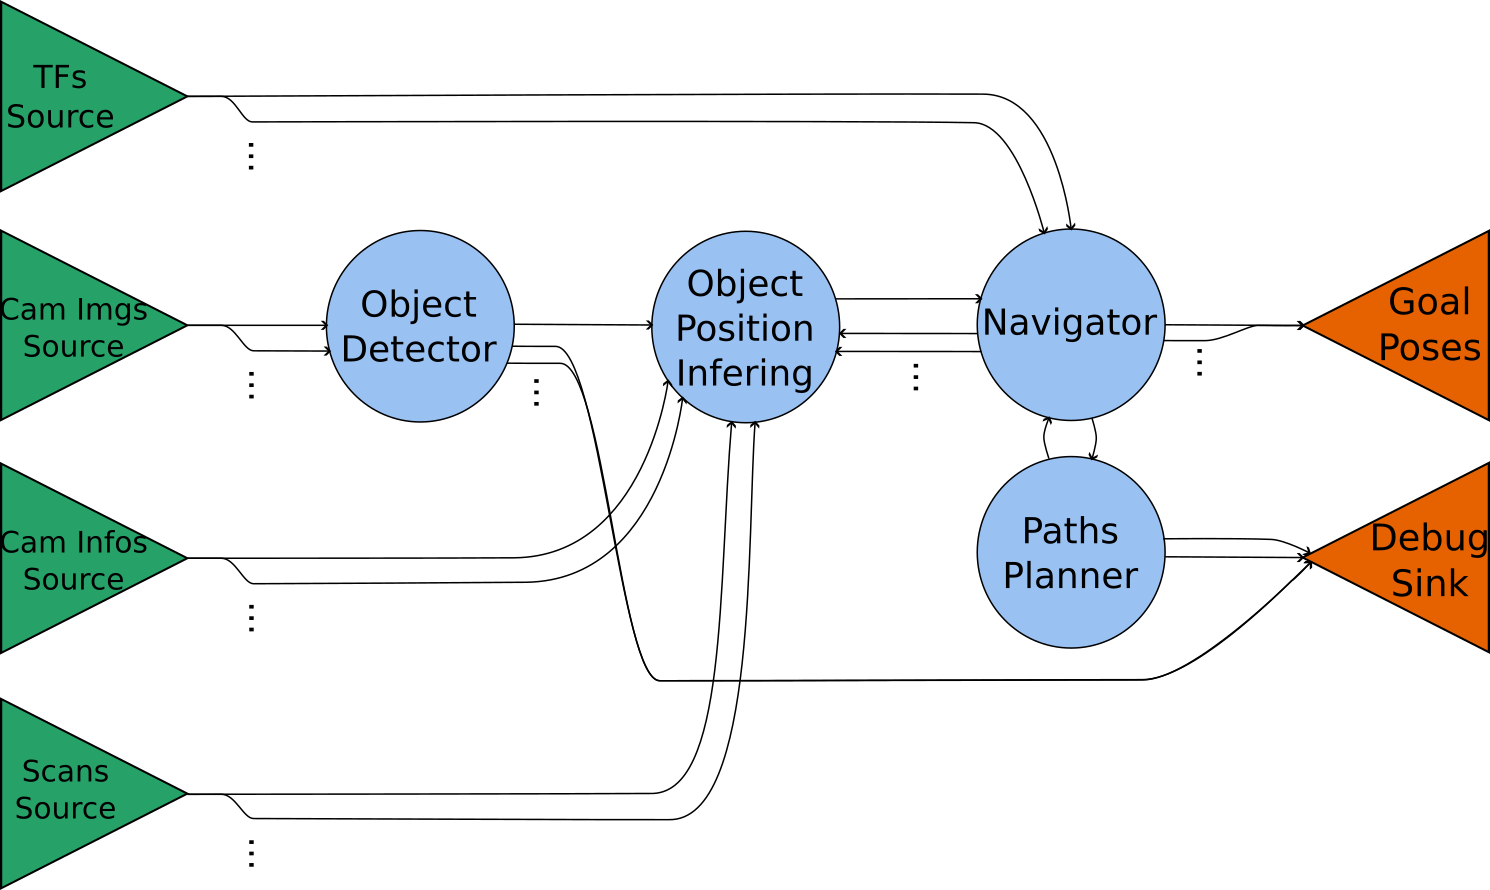
\includegraphics[width=8.0cm]{figs/data_flow_scheme.png}
\end{figure}
\note[item]{Con este contexto podemos visualizar un flujo de datos como una red
de nodos que forman un grafo dirigido, en el que los datos fluyen entre dichos
nodos.}
\note[item]{En la imagen podemos ver un ejemplo de uno de ellos, concretamente
de la aplicacaión desarrollada para este proyecto, basada en la búsqueda de un
objeto en una sala por múltiples robots.}
\note[item]{En concreto, el desarrollo de este proyecto comenzó durante mis
prácticas de empresa en París, en la empresa ZettaScale, desarrolladora de todos
los softwares reliativos a Zenoh que he mencionado, incluído este.}
\end{frame}


\begin{frame}
\frametitle{Pruebas}
\begin{block}{Pruebas en simulación}
\begin{outline}
\1 \textcolor{red}{Correcciones} de nodos de Zenoh-Flow.
  \2 nodo Navigator.
  \2 nodo ObjDetector.
\1 \textcolor{red}{Modificaciones} modelo 3D del Turtlebot 3.
\end{outline}
\end{block}
\begin{figure}
\centering
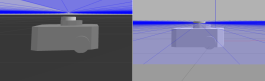
\includegraphics[width=10.0cm]{figs/turtlebot_model_mods.png}
\end{figure}
\note[item]{Desde entonces y durante el desarrollo de este trabajo de fin de
grado se han ido aplicando arreglos de fallos, actualizaciones, correcciones y
mejoras, hasta hacer funcionar correctamente las comunicaciones de red con Zenoh
como protocolo, así como la propia aplicación robótica desarrollada, tanto en
simulación, como en un entorno de laboratorio con robots reales.}
\end{frame}

%[TODO] Añadir vídeos (sim, real, y ¿robots rotando?)
% vdeo resumen: https://youtu.be/JNb0i57Nfjg

\begin{frame}
\frametitle{Pruebas}
\begin{block}{Pruebas de laboratorio}
\begin{outline}
\1 \textcolor{red}{Telecomunicaciones}, (\textcolor{blue}{ROS2}, CycloneDDS, Zenoh API, \textcolor{blue}{Zenoh}, \textcolor{blue}{Zenoh-Flow}, \textcolor{blue}{Zenoh-bridge-DDS}...)
%  \2 ROS2 + CycloneDDS
%  \2 Zenoh API
%  \2 Zenoh + Zenoh-bridge-DDS + ROS2
%  \2 Zenoh-Flow + Zenoh-bridge-DDS + ROS2
\1 \textcolor{red}{Modificaciones} para laboratorio
  \2 Mapas
  \2 Cambios de nombres de frames
  \2 Solución de bugs (nodo PathsPlanner)
\1 \textcolor{red}{Escalabilidad} a 3 robots.
\1 Pruebas con \textcolor{red}{detector de objetos} (nodo \textcolor{blue}{ObjDetector}).
\end{outline}
\end{block}
\begin{block}{}
\begin{outline}
\1 \url{https://youtu.be/JNb0i57Nfjg}
\end{outline}
\end{block}
\note[item]{Con la resolución de distintos fallos se consiguió también llevar la
aplicación al entorno real de laboratorio, con el único problema de que no fue
posible trasladar el nodo de detección debido fallos externos en el software,
relativos a los nodos de ROS2 de las cámaras y a la cola de mensajes del sensor
láser generada por Zenoh-Flow a la hora de comenzar el flujo de datos.}
\end{frame}





\section*{}
\begin{frame}{}
  \centering \Huge
  \emph{Conclusiones}
\note[item]{Para acabar esta presentación, vamos a repasar lo hecho, unas breves conclusiones y las líneas futuras.}
\end{frame}

\section{Conclusiones}
\begin{frame}
\begin{block}{Objetivos cumplidos}
\begin{itemize}
\item Desarrollo de \textcolor{red}{forma de programación de flujos de datos} en conjunto con ROS2.
\item Desarrollo de una \textcolor{red}{aplicación robótica} que lo demuestre.
\item \textcolor{red}{Sencillez} de código y hardware \textcolor{red}{económico}.
\item Solución a la \textcolor{red}{brecha de aprendizaje}.
\end{itemize}
\end{block}

\begin{block}{Líneas futuras}
\begin{itemize}
\item Actualización a \textcolor{red}{versiones más estables}.
\item \textcolor{red}{Paquete} de instalación.
\item \textcolor{red}{Aplicación} con interfaz \textcolor{blue}{sencilla e intuitiva}.
\end{itemize}
\end{block}
\end{frame}

\begin{frame}[plain]
\large{\titlepage}
\note[item]{Y hasta aquí mi exposición.}
\note[item]{Quedo a disposición del tribunal...}
\end{frame}

\end{document}



% [TODO] Hacer diapositivas extra al final para resolver dudas (explicando más a
%        fondo algún tema complejo que tal vez pueda no haber quedado claro).
